
\section{插入图片}

论文中会插入图片\index{图片}、表格\index{表格}等元素。在Word中插图也是一件比较头疼的事,
涉及图的位置布置,大小,清晰度等问题。在\LaTeX 中这些问题也在一定程度上存在,
但\LaTeX 尽可能使得排版出来效果较好。相对于Word,虽然不是所见所得形式,
初期学习比较繁琐,但经短时间熟悉后可以比Word处理快不少。
我最喜欢的方式就是用Octave+gunplot把曲线图做成标准一样的大小,然后把这些图命好名,
放到一个专门的目录中去,一次全插好,如果要修改所有图的大小及式样,只要修改一下相应的Octave的生成曲线脚本文件即可。
这样整篇文档中的曲线图都是统一的模式,统一大小,统一字体,非常整齐。

下面对\LaTeX 中常见的插入图片方法作简要介绍,对于大部分专业做毕业论文应该是足够了,
更多更复杂的方式,有兴趣的可以查找相关专题说明文档\cite{epslatex},
这里提到的文献[\citenum{epslatex}]中给的是英文原版的下载地址,中文版搜一下网上到处有。

\LaTeX 支持的图片格式分两种情况:

\begin{enumerate}

\item{tex-$>$dvi-$>$pdf方式}

包括tex-$>$dvi-$>$ps-$>$pdf这样一个过程,本模版推荐采用的方式是tex-$>$dvi-$>$pdf,
这样的处理流程下,只能采用eps\index{eps}格式的图片。
如果你只有jpg\index{jpg},jpeg,png,gif之类格式的图片,那么不要紧,
\LaTeX 中提供了一个转换程序bmeps.exe\index{bmeps},可以帮助你把jpeg图片转换成eps格式,
当然你也可以用photoshop\index{photoshop},gimp转换。使用bmeps的命令格式如下:

bmeps -p 1 -c picture.jpeg picture.eps

其中,-p 1是压缩出的图片质量,1最好,2是默认,3最差。-c是保留彩色,不带c图片为黑白。

\item{tex-$>$pdf方式}

如果是用pdfTeX\index{pdfTeX}直接将tex转换为pdf的流程,则不能采用eps格式,但可以采用jpg,jpeg,
png,gif这些格式。

如果只有eps格式图片,则可以使用photoshop,gimp或者Acrobat\index{Acrobat}将其转为pdf格式。

这也是为什么这个模版带的文件中既有eps又有pdf的原因,
为了照顾到部分直接将tex转换到pdf的同学。

\end{enumerate}

{\bfseries 本模版推荐新手使用eps格式图片。}
eps格式没使用过\LaTeX 可能会比较陌生,eps也是一种矢量格式\index{矢量}图形。就是说如果是从矢量图形
转到eps格式,一样可以无损缩放。

subsection{图片插入的一般方法}

在文中插入图片的常用命令如下(以使用eps格式为例):

{
\linespread{1}
\zihao{-5}\noindent
\begin{verbatim}
\begin{figure}[htb]
\centering
\includegraphics{picture.eps}
\caption{图片标题}
\label{Figflag}
\end{figure}
\end{verbatim}
}

\verb+\begin{figure}[htb]+是告诉\LaTeX 软件准备插入图片,[htb]是一个选项,
代表图片的插入位置,h代表在文中当前位置,t代表一页的顶部,b代表页面底部,
还有一个选项是p,代表图片要单独放在一页中,如果不给出这些选项,
\LaTeX 会试着依次选用h-t-b-p方式,找出自已认为最合适的,如果给出一选项,
\LaTeX 就只使用给出的一个选项,如果给出几个选项,\LaTeX 会尝试给出的这几个选项,
然后选用它认为最合适的。
一般采用默认方式,不给出任何选项。除非有个把图\LaTeX 自动给出的位置不好,
再通过这几个选项来选择。

\verb+\centering+表示图片的位置为居中放置。

\verb+\includegraphics{picture.eps}+指出了要添加的图片的文件名,
如果图片在其它目录中,比如pictures文件夹,命令则变为:\\
\verb+\includegraphics{pictures/picture.eps}+。\\
要着重说明的是,插入的图片可以采用选项进行缩放\index{缩放},旋转。
比如,要把图片设置为同文字部分一样宽,如图 \ref{FigTextWidth} ,
则命令变为:\\
\verb+\includegraphics[width=\textwidth]{picture.eps}+

\begin{figure}[htb]
\centering

\includegraphics[width=\textwidth]{./Pictures/LHS.eps}
\caption{跟文字一样宽的图}
\label{FigTextWidth}
\end{figure}

指定为与文字一样宽太宽了,下面来把它缩小点,比如半个文字宽度,
那么就用\verb+width=0.5\textwidth+,如果指定10cm宽,就用width=10cm,
如果指定7cm高,就用height=7cm,如果是指定原图大小的50\%,就用
scale=0.5,如果我们想把它调整到原尺寸大小的50\%,再逆时针旋转90度
(如想顺时针旋转则使用负角度值),
就用如下的命令:\\
\verb+\includegraphics[scale=0.5,angle=90]{picture.eps}+\\
效果如图 \ref{FigHalfr90} 所示。

\begin{figure}[htb]
\centering

\includegraphics[scale=0.5,angle=90]{./Pictures/LHS.eps}
\caption{原图一半大小并逆时针旋转90度的图}
\label{FigHalfr90}
\end{figure}

常用的图片调整参数有:width,height,angle,scale这四个,
如果想要更多的效果,比如把图片四边裁掉,像Word中那样。
请参考graphicx\index{graphicx}包的帮助文件graphicx.pdf\footnote{此处要说明一下,
\LaTeX 安装的所有扩展包\index{扩展包}都有对应的说明文档,
请到\LaTeX 的安装目录中寻找,比如本模版使用的MiKTeX2.9的安装文件夹。
帮助文件文件名一般与扩展包名相同,格式为pdf或者dvi,少量的扩展包
帮助文件直接给的tex源文件,需要自行生成文档。}。

\verb+\caption{图片标题}+给出了图名,使用这条命令后,图下方就有了图名。
并且图片目录中也会出现相应的内容。如果图的名字比较长,有可能会造成图片
目录中的目录项换行,类似章节标题命令的格式,增加一个参数哪下:

\verb+\caption[图片目录中的标题]{图片下方出现的标题}+

\verb+\label{FigHalfr90}+这里给出了这个图片的标签“FigHalfr90”,
当你文档中要出现“如图 X.x所示”时,只要写成
“如图\verb+ \ref{相应的图片标签} +所示”即可。\LaTeX 会替你把标签换成图的编号。
这里要注意的是,一是引用命令前后各有一个空格,二是标签不能含有中文字符。

\verb+\end{figure}+表示图片插入结束。

这里提一些题外话,无兴趣研究\LaTeX 的同学请无视此段,
以上使用的图片插入命令并不符合\LaTeX 命令标准,
但是因为其方便应用,成为了应用最广泛的\LaTeX 命令。
标准的命令格式在graphicx.pdf中有详细说明。
另外,\LaTeX 还有一个图形扩展包,叫做graphics\index{graphics},注意最后一个字母,
一字之差,graphics包支持的功能更多一些,但大部分普通应用应用不到,
而且,graphics只支持标准命令调用。有兴趣的同学可以研究一下graphics.pdf,
此处我就不再多说了。

\subsection{插入图片的应用进阶}

刚才前面有提到:eps是一种矢量格式图形,所谓矢量格式图形,
就是放大缩小都会会造成图片变“糊”。其实,eps的方便之处还不止这些,
大部分的科学计算软件都支持生成eps格式图片,比如matlab,可以直接生成
eps格式图片。

有同学会说,那我用Microsoft Visio画的图怎么处理呢?Visio创建的图形也是矢量图,
在Word下是可以任意缩放的。如果你装有ps虚拟打印机或者acrobat,
这个问题就迎刃而解了。首先选中你要打印的visio图形,然后把它打印成ps或者pdf文档。
接下来ps文档的话就直接用安装CTeX组件时带的Ghostscrip转换成EPS图像,
pdf文档的话就先用Acrobat打开,菜单-工具-高级编辑-裁剪工具,
把所需要的图形那一部分剪出来,另存为eps文件即可。用photoshop同样可以达到这个效果。
这样出来的图像依然是矢量图,可以任意缩放不会糊。

\LaTeX 通过使用psfrag扩展功能包,还能对eps中的一些字符进行替换。
但是遗憾的是,psfrag只支持dvips转换程序,
本模版推荐使用的dvipdfm程序不支持该扩展包。
但这不要紧,我们可以采用变通的方法,把要替换字符的图用
tex-$>$dvi-$>$ps-$>$pdf的流程处理,
再生成的pdf用Acrobat裁剪后生成eps文件即可。

参考代码如下,生成图片效果对比如图 \ref{Figmatlab} 所示:

{
\linespread{1}
\zihao{-5}\noindent
\begin{verbatim}
\documentclass{article}
\usepackage{graphicx}
\usepackage{psfrag}
\begin{document}
\pagestyle{empty}
\psfrag{s1}{$y=sinx$}
\psfrag{x}{$x$}
\psfrag{y}{$y$}
\includegraphics{matlabfig.eps}
\end{document} 
\end{verbatim}
}

\begin{figure}
\centering
\includegraphics[scale=0.6]{./Pictures/matlabfig.eps}
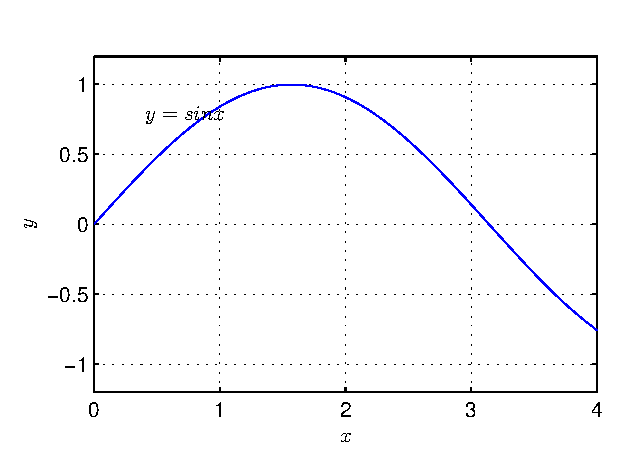
\includegraphics[scale=0.6]{./Pictures/matlabfigchg.eps}
\caption{matlab作图例}
\label{Figmatlab}
\end{figure}

图 \ref{Figmatlab} 中左图为matlab生成的eps图,右图为将左图中的s1,
纵横坐标名替换后的图片。可以把这一页放大几倍来看,图片依然非常清晰!
这就是矢量图的优势。
替换文字中如果有中文出现,因为dvips程序与cjk不兼容,
本论文模版的tex-dvi-pdf生成方式将不能用于含有dvips流程,使用dvips须使用cct方式,
具体请参考CTeX FAQ,有详细例子。

\subsection{子图的使用}
有些时候我们需要使用一级图放到一个大图中,这次版本也提供这种支持,具体实现代码如下:

{
\linespread{1}
\zihao{-5}\noindent
\begin{verbatim}
\begin{figure}[htb]
	\small
	%\centering
	\subfigure[子图1]{
		\begin{minipage}[b]{0.5\textwidth}
			\centering
			\label{fig:SubFigure1} %% label for second subfigure
			\includegraphics[scale=0.6]{./Pictures/matlabfig.eps}
		\end{minipage}}
		\subfigure[子图2]{
			\begin{minipage}[b]{0.5\textwidth}
				\centering
				\label{fig:SubFigure2} %% label for second subfigure
				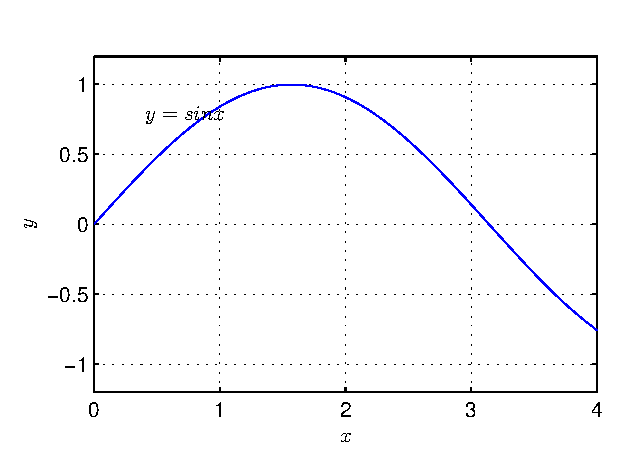
\includegraphics[scale=0.6]{./Pictures/matlabfigchg.eps}
			\end{minipage}}
			\caption{两个子图示例}
			\label{Fig:SubFigures}
		\end{figure}
\end{verbatim}
}
实现效果如图\ref{Fig:SubFigures}所示。

\begin{figure}[htb]
	\small
	%\centering
	\subfigure[子图1]{
		\begin{minipage}[b]{0.5\textwidth}
			\centering
			\label{fig:SubFigure1} %% label for second subfigure
			\includegraphics[scale=0.6]{./Pictures/matlabfig.eps}
		\end{minipage}}
	\subfigure[子图2]{
		\begin{minipage}[b]{0.5\textwidth}
			\centering
			\label{fig:SubFigure2} %% label for second subfigure
			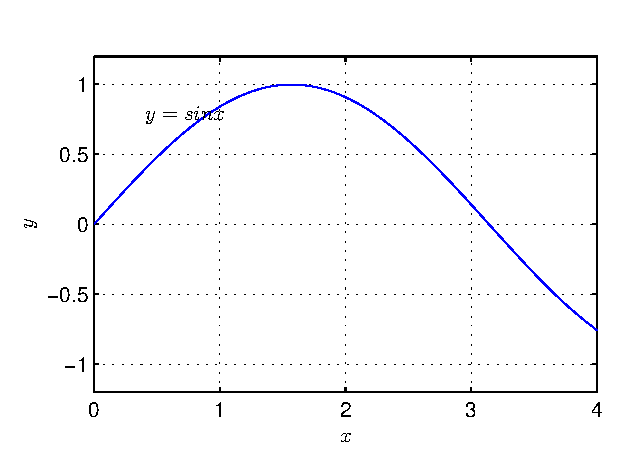
\includegraphics[scale=0.6]{./Pictures/matlabfigchg.eps}
		\end{minipage}}
		\caption{两个子图示例}
		\label{Fig:SubFigures}
\end{figure}

\section{插入表格}

\LaTeX 中建立表格比Word稍复杂一些,但表格的格式调整及效果比Word简单得多。

\subsection{普通表格的插入}

一个普通的插入表格代码如下所示,其生成的表格如表 \ref{Tabkeyword} 所示:

{
\linespread{1}
\zihao{-5}\noindent
\begin{verbatim}
{
\begin{table}[htb]
\zihao{5}
\caption{表格标题}
\label{Tabkeyword}
\centering
\begin{tabular}[t]{c|l|r|p{4cm}}
\hline
居中 & 靠左 & 靠右 & 靠左宽4cm\\
\hline
Center & Left & Right & Width=4cm\\
\hline
\end{tabular}
\end{table}
}
\end{verbatim}
}

\begin{table}[htb]
\zihao{5}
\caption{表格标题}
\label{Tabkeyword}
\centering
\begin{tabular}[t]{c|l|r|p{4cm}}
\hline
居中 & 靠左 & 靠右 & 靠左宽4cm\\
\hline
Center & Left & Right & Width=4cm\\
\hline
\end{tabular}
\end{table}

表格的使用一部分与图片相类似,比如开始的语句\verb+\begin{table}[htb]+,
以及结束的语句\verb+\end{table}+,与图片语句相比,除了把“figure”换成了
“table”,其它都相同。语句的含义也相同。

\verb+\zihao{5}+是把表格的字号改小一号,一般而言,表格字号应比正文字号小一号,
论文中的正文字号是小四号,那么表格中的字号就应该是五号字体。这个命令一定要写在
\verb+\begin{table}+ 的下方才能对该表格起作用。

\verb+\caption{表格标题}+是表格的标题,与图片标题格式相同,
会自动加到表格目录中去,如果表格标题太长,可以用
\verb+\caption[目录中的标题]{正文中的表格标题}+这种形式。

\verb+label{Tablekeyword}+与图片的标签相同,只要在正文中使用\\
\verb+\ref{Tablekeyword}+ 就可以在生成的文档中显示出表的编号,
同样,命令前后要各留一个空格,并且标签不能使用中文字符。

\verb+\centering+ 使整个表格居中放置。

\verb+\begin{tabular}[t]{c|l|r|p{4cm}}+是表格开始的标志,注意与
\verb+\begin+ \verb+{table}+区别开来,\verb+[t]+表示表格与其上方的正文行对齐方式是
行顶对齐,如果是\verb+[b]+则为行底对齐,这两种对齐方式可以在实际操作中试一下,
再做选择。\verb+{c|l|r|p{4cm}}+则代表这个表格各列的
对齐方式,c为居中,l为左对齐,r为右对齐,p\{4cm\}为该列宽度为4cm,并且左对齐。
中间接竖线“\verb+|+”则表示表格使用竖分隔线,如果没有这个竖线符号,对应位置就没有分隔线,
比如表 \ref{Tabkeyword} 就没有最左边和最右边的竖线。如果写为\verb+{|c|l|r|p{10cm}|}+,
就有最左边和最右边的竖线了。
如果不需要竖分隔线,则写为\verb+{clrp{10cm}}+
即可。要使用双竖线分隔线,就写为\verb+{c||c}+;还可以使用其它字条代替,
比如本模版的题名页中评阅人及答辩委员会信息就是利用的表格形式,它的分隔符是冒号“:”,
相应的命令就是\verb+{c@{:}c}+,即\verb+@{:}+。

\verb+\hline+就是画一条横线,如果没有写这一句命令,你会看到表格没有横分隔线。

表格内容是一行一行来填的,每一行结束使用断行符\verb+\\+,
同一行中不同列的元素用\&来分开。

\verb+\end{tabular}+表示表格结束。

\subsection{把表格换个样式}

上一小节介绍的方法生成的表格一般情况下可以用了,
但\LaTeX 的能力不止是做这样一个常规表格,
下面我们来利用booktabs-de\index{booktabs-de}扩展包来让表格看起来更professional一些。
这个扩展包的调用已经放在了本模版中了,使用本模版可以直接使用这种格式。
这个表格如表 \ref{Tab3Line} 所示。

{
\linespread{1}
\begin{table}[htb]
\zihao{5}
\caption{粗细线表格示例}
\label{Tab3Line}
\centering
\begin{tabular}[b]{cccc}
\toprule
长 & 宽 & 高 & 重量\\
(m) & (cm) & (mm) & (kg)\\
\toprule
1.234 & 5.676 & 332.876 & 3498.5\\
\midrule
548.4 & 23.43 & 34.98 & 923.8\\
\bottomrule
\end{tabular}
\end{table}
}

表 \ref{Tab3Line} 的实现代码如下所示:

{
\linespread{1}
\zihao{-5}\noindent
\begin{verbatim}
{
\linespread{1}
\begin{table}[htb]
\zihao{5}
\caption{粗细线表格示例}
\label{Tab3Line}
\centering
\begin{tabular}[b]{cccc}
\toprule
长 & 宽 & 高 & 重量\\
(m) & (cm) & (mm) & (kg)\\
\toprule
1.234 & 5.676 & 332.876 & 3498.5\\
\midrule
548.4 & 23.43 & 34.98 & 923.8\\
\bottomrule
\end{tabular}
\end{table}
}
\end{verbatim}
}

先解释一下这部分代码为什么会用一对大括号\{\}整个括起来。
如果要对文章中一部分内容的格式作调整,又不能影响到其它部分,
就使用一对大括号把要调整格式的部分括起来。
这里要调整的格式是行距。本论文的默认行距是1.5倍行距
\footnote{模版中的行距调整命令是$\backslash$linespread\{1.5\},
但并不是直接的1.5,这里有个换算,有兴趣的同学可以查看参考文献\cite{LaTeXshzh}},
在这里要把它调成单倍行距这个表格样式才比较美观,
因此就在最前使用\verb+\linespread{1}+命令把它的行距调整为单倍行距。
关于局部格式调整,在后面的《重点字符,醒目提醒》
一节中还将详细介绍,这里只对牵涉部分做简要说明。

这部分代码与普通表格代码的区别在于横线生成命令:\verb+\toprule+,\verb+\bottomrule+
都是比较粗的线条,\verb+\midrule+是比较细的线条。
此外,还有一个不完整线条命令,\verb+\cmidrule+,
该命令的使用类似下一小节要讲到的\verb+\cline+命令。

\subsection{有单元格合并的表格}

表格不可能总是一格归一格的。部分表格总是需要进行表格合并,
下面我就举一个表格合并的例子。\LaTeX 直接支持列合并,行合并则需要
扩展包multirow\index{multirow}的支持,本模版已经将该扩展包包含进去,可直接使用。
如表 \ref{TabComplex} 所示表格

\begin{table}[htp]
\zihao{5}
\caption{复杂表格示例}
\label{TabComplex}
\centering
\begin{tabular}[t]{|c|c|c|c|c|}
\hline
\multicolumn{2}{|c|}{我占了两列} & 第3列 & 第4列 & 第5列\\
\hline
\multirow{2}*{我占了两行} & 第二行第2列 & 第二行第3列 & \multicolumn{2}{|c|}{\multirow{2}*{我占了两行又两列}}\\
\cline{2-3}
& 第三行第2列 & 第三行第3列 & \multicolumn{2}{|c|}{} \\
\hline
\end{tabular}
\end{table}

表 \ref{TabComplex} 的实现代码如下:

{
\linespread{1}
\zihao{-5}\noindent
\begin{verbatim}
\begin{table}[htp]
\zihao{5}
\caption{复杂表格示例}
\label{TabComplex}
\centering
\begin{tabular}[t]{|c|c|c|c|c|}
\hline
\multicolumn{2}{|c|}{我占了两列} & 第3列 & 第4列 & 第5列\\
\hline
\multirow{2}*{我占了两行} & 第二行第2列 & 第二行第3列 & \multicolumn{2}{|c|}{\multirow{2}*{我占了两行又两列}}\\
\cline{2-3}
& 第三行第2列 & 第三行第3列 & \multicolumn{2}{|c|}{} \\
\hline
\end{tabular}
\end{table}
\end{verbatim}
}

\verb+\multicolumn{2}{|c|}{表格内容}+就是合并列的命令,参数2表示合并两列,
格式命令表示合并后的单元格居中对齐且两边有分隔竖线,注意在有分隔线时,分隔线符号
\verb+|+不要忘记。

\verb+\multirow{2}*{表格内容}+是合并行的命令,参数2表示合并两行,注意中间的*号。

注意同时合并行合并列时两个命令的嵌套方式,以及合并行情况下,除第一行外其它行的表示方式。
如合并两行两列时第二行的\verb+\multicolumn{2}{|c|}{}+。

\verb+\cline{2-3}+代表横线只划第二列与第三列,如果划2,3,5列,则写为\verb+\cline{2-3,5}+
\verb+\cmidrule+用法同\verb+\cline+。

\subsection{其它高级表格格式及扩展包简介}

如果需要实现表格左上角内有斜线的样式,
请使用slashbox\index{slashbox}扩展包并参考其自带帮助文档。

更复杂的表格,比如指定每一行的宽度,即可以借助盒子\cite{LaTeXshzh}来完成,
也可以借助扩展包array,tabularx等,具体实现代码此处不再详述,有兴趣的同学可参考文献
\cite{LaTeXshzh, Table:Lapo}以及扩展包内帮助文件。

\section{公式及其编号}

\LaTeX 出现之初的重要作用就是排版各种复杂的数学公式,关于数学公式的排版方法,
参考文献\cite{LaTeXshzh}中有一整章的内容来介绍各种公式的编辑。
我这里就偷个懒不写了,太长了,而且公式编辑我写不出我的特色来。

\LaTeX 的公式编辑效果远胜于Word中的公式编辑器,而且,使用LaTeX,
完全不用担心公式编辑器的版本问题,因为,这里公式就是用纯文本写的。
下面我举一个小小的公式例子来说明公式的编写及编号,如式 \ref{Equ:exm} 所示。

\begin{equation}
\label{Equ:exm}
c^2=a^2+b^2
\end{equation}

实现式 \ref{Equ:exm} 的代码如下所示:

{
\linespread{1}
\zihao{-5}\noindent
\begin{verbatim}
\begin{equation}
\label{Equ:exm}
c^2=a^2+b^2
\end{equation}
\end{verbatim}
}

\verb+\begin{equation}+与图片,表格很类似,开头都是一个环境开始命令,
只是这里的关键词是equation\index{equation}。

\verb+label{Equ:exm}+是给公式一个编号,以便在文中引用。该公式编号由\LaTeX 负责,
一般不需人工干预。

\verb+\ref{Equ:exm}+就是文中引用公式的命令。

\section{索引}

索引比较简单,只要在你想放索引的位置放上命令\\
\verb+\index{索引名}+,\\
然后文后面的索引列表中就出现“索引名”这个条目,并且有它的页码,
索引支持中文,英文字符。
如果文中有多处同名索引,这个表中都会把它们按字母表顺序列出来。
很方便的,你想在哪里插入索引就在哪里插入索引,完全不必考虑索引列表的事。

\section{参考文献}

前面介绍参考文献时就提到,只要准备好自己的参考文献数据库,
在引用参考文献时只需要利用\verb+\cite{tag}+就能把相应的参考文献引上。
这里的tag就是在参考文献数据库中各参考文献定义的标签,不能含有中文字符。
多个文献,则中间用英文逗号分开如\verb+\cite{tag1,tag2}+。
不需要考虑引用顺序,\LaTeX 会替你打理好一切。

如果想用形如“文献[1]提出XXX”的格式,则使用如下代码。

{\noindent\zihao{-5}\verb+文献[\citenum{tag}]提出+}

该模版已经把各类参考文献的列出格式按毕业论文要求调整好,不需要再修改。

如果你想了解更多参考文献格式调整的信息,请参考扩展包natbib\index{natbib},custom-bib\index{custom-bib}
自带的帮助文档。本次修订版新增的第5章也专门会对参考文献的格式校调问题进行大篇幅介绍。

\section{脚注}

有些时候需要使用脚注,\LaTeX 的脚注功能也是很方便的,
只要在你想要放一个脚注的地方用命令\verb+\footnote{脚注内容}+即可,
脚注内容长度不限,脚注编号\LaTeX 会替你操心。
你要做的,只是写好这个脚注的内容。

对于表格加脚注,就像表 \ref{ChapsecList} 显示效果那产,则稍显麻烦一点,需要把表格放进一个minipage里去。
关键代码如下:

{
\linespread{1}
\zihao{-5}\noindent
\begin{verbatim}
\begin{table}
……
\centering
\begin{minipage}[c]{10cm}
\centering
\begin{tabular}
……
\end{tabular}
\end{minipage}
……
\end{table}
\end{verbatim}
}

\verb+\begin{minipage}[c]{10cm}+表示创建一个内部居中对齐的,
宽度为10cm的小页面,这个宽度要根据其内部表格宽度来确定,
这样出来的脚注才美观。

\section{重点字符,醒目标示}

有的时候需要对某些内容做一个醒目标示,比如改变字体啦,字体加粗啦。
这个时候首先要把需要改变格式的部分用一对大括号
\footnote{要使用英文字符的大括号\{\}}括起来。
然后在头上写上字体字号之类的命令。就像这样

我这一段话里有{\bfseries 加粗},
{\kaishu\bfseries 有楷体并加粗},有{\heiti 黑体},还有{\zihao{3}三号字}字体。

这一句话的实现代码如下:

{
\linespread{1}
\zihao{-5}\noindent
\verb+我这一段话里有{\bfseries 加粗},{\kaishu\bfseries 有楷体并加粗},有{\heiti 黑体},还有{\zihao{3}三号字}字体。+
}

%在\LaTeX 中可以用的字体有{\songti 宋体}\verb+\songti+,{\fangsong 仿宋}\verb+\fangsong+,
%{\kaishu 楷体}\verb+\kaishu+,{\heiti 黑体}\verb+\heiti+,
%{\youyuan 幼圆}\verb+\youyuan+,{\lishu 隶书}\verb+\lishu+六种。字号命令是\verb+\zihao{1}+字号从
%1,-1,2,-2,一直到8号字,前面带负号表示小号字,比如-4就是小四号字体。
%7,8两个字号没有小号字对应。

关于加粗字体命令\verb+\bfseries+,对英文字符只要使用\verb+\bf+即可,
中文字符应使用\verb+\bfseries+。

关于字体效果的设置,更多内容参见CTeX自带的帮助文档ctex.pdf。

如果想使用更多的字体,比如微软雅黑,请自行网络搜索方法,自己生成字体文件并关联上即可。
CTeX提供的六种字体,一般情况下已经足够使用。


